%%%%%%%%%%%%%%%%%%%%%%%%%%%%
% OLD TEXT : Use in thesis %
%%%%%%%%%%%%%%%%%%%%%%%%%%%%

Here we calculate the probability of detecting a new point source as a
function of magnitude.  We use a Monte Carlo simulation in which
artificial point sources of various magnitudes are added to survey
images. The images are then run through the same reduction and SN
detection pipeline used in the search.

Because our search procedure uses information from individual
exposures to reject cosmic rays, it is necessary to place the
artificial point sources on these individual exposure images rather
than on the combined image from each visit. This allows us to test
both the efficiency of the {\sc MultiDrizzle} process and our CR
rejection. We add the artificial point sources to the raw CCD images
after bias subtraction and flat fielding. As these ``\texttt{\_flt}''
images have not been re-sampled, they accurately represent the light
on each CCD pixel.

As a model of the point spread function (PSF) on these images, we use
the PSF library of \citet{anderson06a}. For each of six ACS filters,
this library represents the position-dependent PSF by a $9 \times 10$
array of fiducial PSFs across the two CCDs. Each fiducial PSF model is
oversampled by a linear factor of 4, giving the model a pixel scale of
$0''.0125$. As this library was derived on \texttt{\_flt} images, it
is directly applicable to these images.

The artificial point sources are placed on galaxies according to the
distribution of light in each galaxy. Galaxies with $z_{850} < 20$ are
not used, as these are only found at redshifts below the range of
interest. Only one point source is placed on each galaxy to avoid
detection complications from overlapping sources.  Once a position on
a galaxy is chosen, it is converted to a corresponding CCD chip
position on each of the (typically four) individual exposure images
taken for the visit.  The oversampled fiducial PSF model for this
position on the CCD is chosen from the PSF library and is re-sampled
onto the CCD pixels. A random point source flux is drawn from the
range of interest. The PSF model is adjusted to match this flux. It is
normalized so that the encircled energy in a 3~pixel radius aperture
in the combined image matches the value derived
by \citet{sirianni05a}.  A further adjustment to the flux is made to
compensate for the variation in effective pixel area across the
detector. (This variation is due to the ACS distortion and is on the
order of 10 to 20\%.) Poisson noise is added to each pixel in the PSF
and the PSF is then added to the image.  Images are passed through the
same reduction and detection pipeline used in the search. Finally, the
flagged candidates are compared to the input artificial point sources.

%%%%%%%%%%%%%%%%%%%%
% PLOT: EFFICIENCY %
%%%%%%%%%%%%%%%%%%%%
\begin{figure}[t]
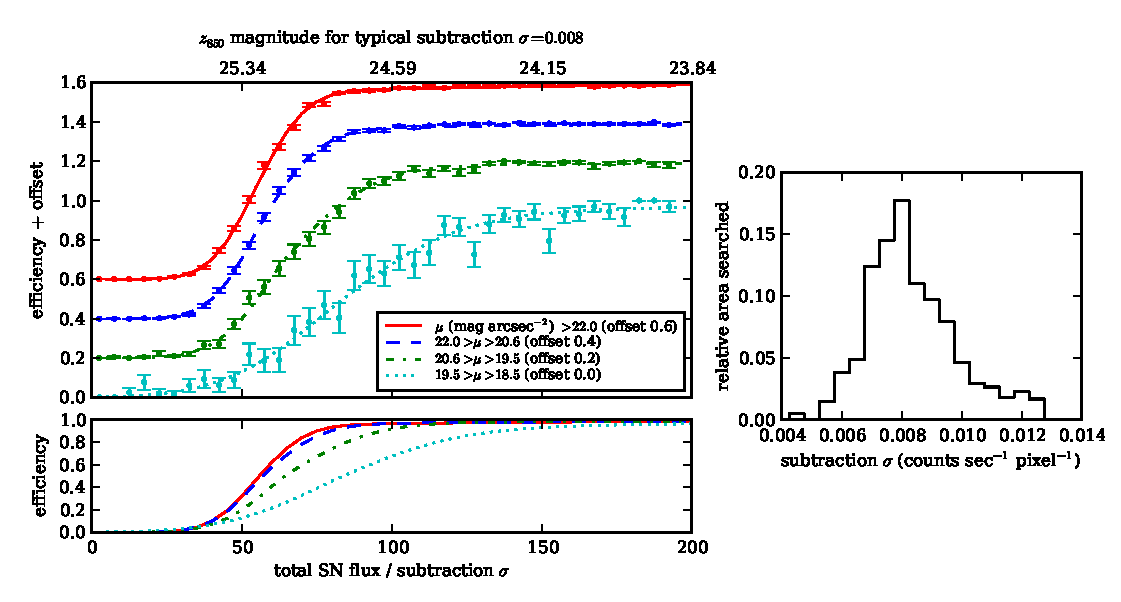
\includegraphics[width=\textwidth]{figures/clrate/eff_color.eps}
\caption[Point source detection efficiency]{Point source detection 
efficiency in a single subtraction, 
as a function of the ratio of total point source flux to subtraction
noise $\sigma$ (counts~sec$^{-1}$~pixel$^{-1}$). The artificial point
sources are split into four bins depending on the underlying galaxy
surface brightness $\mu$ (mag~arcsec$^{-2}$) at the point source
position. The efficiency curve is calculated separately for each
bin. In the \emph{upper left panel}, the four bins are shown, offset for
clarity. In the \emph{lower left panel}, the fitted curves are reproduced
without offset for comparison. Approximately 72,000 artificial point
sources were used in total. The \emph{right panel} shows the distribution of
the noise level in the subtractions. The noise level differs by a
factor of about two from the deepest to shallowest subtractions
searched.\label{fig:eff}}
\end{figure}

%The detection efficiency
%The noise level varies between subtractions and between different
%regions within a single subtraction.  To avoid running a full Monte
%Carlo simulation for each of these subtractions and regions, 

We parameterize the detection efficiency by the ratio of point source
flux to sky noise. This is a good choice because, in most cases, the
detection efficiency will depend only on the contrast between the
point source and the sky noise. However, there is an additional
dependence on the surface brightness at the location of the point
source: point sources near the core of galaxies will have a lower
detection efficiency due to additional Poisson noise from the
galaxy. For $0.6<z<1.5$ galaxies, we estimate that only $\sim$$10\%$
of SNe will fall on regions where galaxy Poisson noise is greater than
the sky noise (assuming SNe follow the galaxy light
distribution). Still, we take this effect into account by splitting
our sample of artificial point sources into four bins in underlying
surface brightness. The detection efficiency is calculated separately
in each bin (Fig.~\ref{fig:eff}, top left panel).  The first two bins,
$\mu > 22.0$ and $22.0 > \mu > 20.6$ mag~arcsec$^{-2}$, correspond to
lower surface brightnesses where sky noise is dominant. As expected,
their efficiency curves are very similar. In the third and fourth
bins, corresponding to higher surface brightness, the Poisson noise
from the galaxy dominates the sky noise, and the efficiency drops as a
result.

For reference, the distribution of sky noise in the subtractions is
shown in Figure~\ref{fig:eff} (right panel). Nearly all the searched
area has a sky noise level between 0.006 and
0.012 counts sec$^{-1}$ pixel$^{-1}$. For a typical value of 0.008, we
show the corresponding point source $z_{850}$ magnitude on the top
axis of the left panel.

We find that the efficiency curve in each bin is well-described by
the function
\begin{equation}
\eta(x) = \left\{ \begin{array}{ll}
\frac{1}{2} (1+ae^{-bx}) [\mathrm{erf}((x-c)/d_1)+1], & x<c     \\
\frac{1}{2} (1+ae^{-bx}) [\mathrm{erf}((x-c)/d_2)+1], & x \ge c
\end{array} \right. ,
\end{equation}
where $x$ is the ratio of point source flux to sky noise, and $a$,
$b$, $c$, $d_1$ and $d_2$ are free parameters. An error function is
the curve one would expect with a constant cut and Gaussian noise, but
we find that two different scales ($d_1$ and $d_2$) in the error
function, as well as an additional exponential term, are necessary to
describe the slow rise to $\eta =1$ at large $x$. This slow rise is
due to rarer occurrences, such as cosmic rays coinciding with new point
sources. The fitted functions for the four bins are plotted in the top
left of Figure~\ref{fig:eff} and reproduced in the bottom left of the
figure for comparison. We use these fitted functions to calculate the
effective visibility time in the following section. 
